\section{История вопроса}

В настоящее время известно много устройств для сбора пчелиного яда. По принципу раздражения пчел они разделяются на механические и электрические.

\subsection*{Механический способ}

Большинство модификаций механического способа раздражения пчел для взятия ядовитого секрета сопровождается гибелью пчел. Для получения яда живые пчелы берутся пинцетом или пальцами, жало при этом высовывается наружу. Тонким глазным пинцетом оно слегка извлекается из камеры, после чего начинается автомати­ческое истечение яда. Кончиком жала прикасаются к поверхности стекла, яд изливается на него и быстро засыхает.

Все устройства, основанные на механическом принципе раздра­жения пчел, имеют ряд существенных недостатков:
\begin{enumerate}
	\item В большинстве устройств и приспособлений для сбора яда пчелы гибнут из-за отрыва ядовитой железы; 
	\item Крайне низкая эффективность устройств, осложненная высо­кой трудоемкостью процесса;
	\item Сбор яда в жидкую среду, где он нестоек, быстро подвергает­ся бактериальному распаду и теряет активность (Артемов Н. М., 1969);
	\item Высокая вероятность поражения (ужаления) пчелами обслужи­вающего персонала.
\end{enumerate}

\subsection*{Электрический способ}

Подлинный переворот в технологии получения пчелиного яда произошел, когда в качестве раздражителя был применен электрический ток. Дело в том, что в основе всех рефлекторных физиологических реакций организма человека и животных лежат электрические, точнее - биоэлектрические процессы, то есть метод электрического раздражения удобен тем, что электрический импульс, наносимый на живую ткань извне, будет адекватным, физиологическим раздражителем. Можно подобрать сигнал такой величины и формы, чтобы он вызвал раздражение, приводящее к ужалению, но не был бы опасен для жизнедеятельности пчелы.

Современный комплекс аппаратуры для получения пчелиного яда включает два основных компонента - электрический стимулятор и ядоприёмник.

Электрический стимулятор представляет собой генератор импульсов тока определенной величины и формы.

Ядоприемник является вторым неотъемлемым компонентом комплекса и представляет собой систему близко расположенных между собой проводов-электродов, через которые импульсы со стимулятора доводятся до тела (конечностей) пчелы. Под проводами-электродами обычно находится стекло - собственно ядоприёмник (см. рисунок. \ref{img:poison_reciever}). Пчела, находящаяся на проводах-электродах, замыкает их в цепь и принимает удар импульсного тока. Возникающая при этом реакция ужаления приводит к тому, что с выдвинутого из брюшка пчелы жала стекает ядовитый секрет, который при высыхании и представляет собой сухой пчелиный яд.

\begin{figure}[h]
  \center{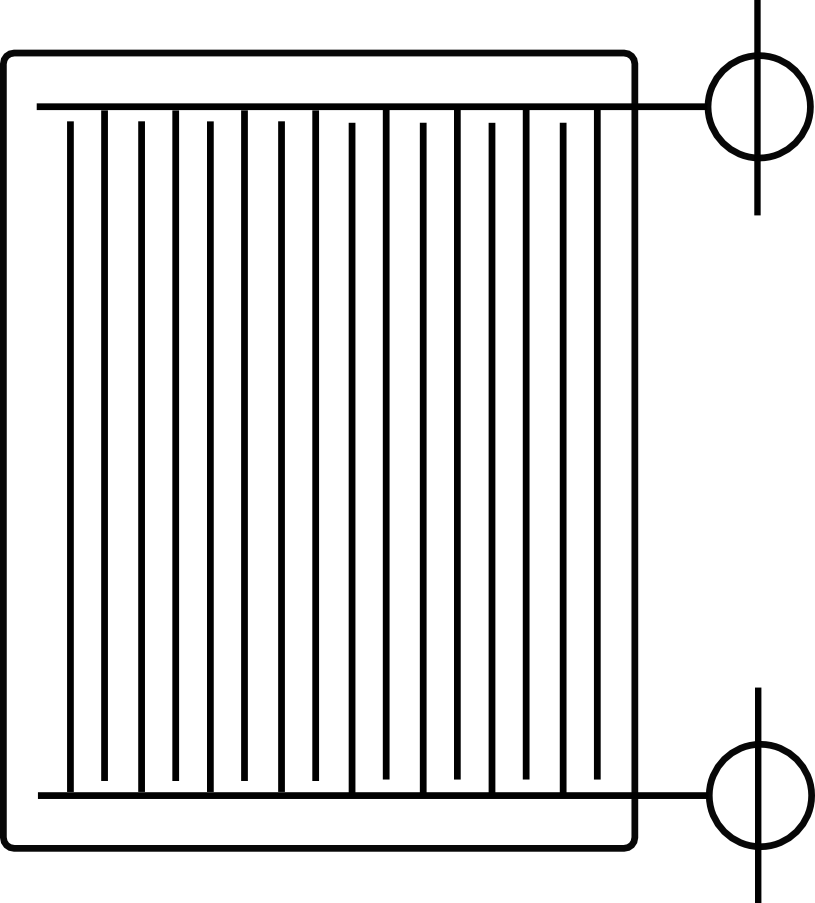
\includegraphics[width=0.25\textwidth]{Images/poison_reciever_scheme.png}}
  \caption{Схематичное представление ядоприемника}
  \label{img:poison_reciever}
\end{figure}

\subsection*{Биологическая составляющая}

Пчела, как и другие животные, имеет центральную и периферическую нервную системы, мышцы, которыми эти системы управляют. Управляющие команды нервной системы регулируются сигналами, приходящими по чувствительным нервным путям от рецепторов, находящихся повсеместно - внутри и на поверхности организма.

Рассмотрим пример. Если несильно надавить на тело пчелы, она будет поднимать лапки, крылья. Если давление усилить - пчела попытается улететь. Наконец, сильное надавливание приведет к попытке ужалить. Следовательно, эти инстинктивные рефлексы и соответствующие реакции градуальны и зависят от раздражающего действия, то есть пчела будет жалить только при достижении определенной, пороговой силы раздражителя.

Установлено, что оптимальным будет раздражение, наносимое в режиме импульсов, причем частота этих импульсов должна соответствовать физиологической частоте. Опытным путем определено, что оптимальная частота электрических импульсов раздражения пчел должна лежать в интервале 500-1000 Гц[Крылов, пчелиный яд].

Стоит заметить, что чем медленнее нарастает величина электрического раздражителя, тем выше становится порог, при котором возникает реакция на раздражение (явление аккомодации). Наоборот, мгновенно нарастающий стимул вызовет реакцию ткани при меньшей величине. Поэтому наиболее эффективны электростимуляторы, у которых передний фронт (крутизна) импульса наиболее короток (0,5-1 мс) - генераторы прямоугольных импульсов.

Важным фактом является то, чтобы получить ответную реакцию пчелы на раздражение, нужно подать пачку импульсов, а не одиночный импульс. Поскольку, при одиночном стимуле даже большой силы мышца отвечает одиночным сокращением.

С другой стороны, для полного выброса яда из мышечного резервуара, мышцы его стенок должны работать в режиме насоса - переодическом сокращении и ослаблении. Соответственно должны быть предусмотрены паузы между пачками импульсов.

Как утверждает автор в [крылов пчелиный яд], в условиях пасеки было подтверждено, что при вышеуказанных параметрах длительности и формы импульсов оптимальная амплитуда составила 25-35 В. При достижении величины в 80 В происходит гибель пчёл на электродах. Также было подтверждено, что повышение амплитуды импульсного тока выше 35 В не приводило к дальнейшему увеличению ядоотдачи.